\chapter*{Tutorial 3}

Create a new struct to send and receive from Server and Client.

\section{Client}
\begin{verbatim}

In the file "AaronMR_Robotic_Stack/Drivers/CB_TCP_RTAI/include/TCP_RTAI/comStruct.h" create a new struct:

  struct posWheels_t
  {
    Point pos_W[4];
  };


In the file "AaronMR_Robotic_Stack/Drivers/CB_TCP_RTAI/include/TCP_RTAI/structType_C.hpp", create a new subclass:

class struct_posWheels : public structType {

public:
    posWheels();
    int serialize(char* data2s);
    int Unserialize(char* data2us);
    void* set_Publisher(char* name);
    void* set_Subscriber(char* name);

    ros::NodeHandle n;
    ros::Publisher posWheels_pub;
    ros::Subscriber posWheels_sub;

    // struct to send and receive
    posWheels_t data2send;
    posWheels_t data2recv;

    geometry_msgs::Point point_msg;
    void cmdCallback(const geometry_msgs::Point &data_);
    bool haveSubscriber;
    bool havePublisher;
    pthread_mutex_t mutex;
    bool canRecv_t;
    bool canSend_t;
    bool canSend();
    bool canRecv();
    int spinOnce();
};


create a new file for the new class, "struct_posWheels.cpp" with the content:

#include "pack2.hpp"
#include "structType_C.hpp"

struct_posWheels::struct_posWheels()
{

}

void struct_posWheels::cmdCallback(const geometry_msgs::Point &data_)
{

}

void* struct_posWheels::set_Subscriber(char* name)
{

}

void* struct_posWheels::set_Publisher(char* name)
{

}

bool struct_posWheels::canSend()
{

}

bool struct_posWheels::canRecv()
{

}

int struct_posWheels::spinOnce()
{

}

int struct_posWheels::serialize(char* data2s)
{

}

int struct_posWheels::Unserialize(char* data2us)
{

}


In the constructor:

struct_posWheels::struct_posWheels()
{

    haveSubscriber  = false;
    havePublisher   = false;
    canRecv_t       = true;
    canSend_t       = true;
    mutex           = PTHREAD_MUTEX_INITIALIZER;

}


Configure the functions to serialize and unserialize:

int struct_posWheels::serialize(char* data2s)
{
   
    unsigned char buf[1024];
    unsigned char magic;
    unsigned int packetsize;
    unsigned int ps2;

    posWheels_t aux;

    aux.pos_W[0].x = 0.0;
    aux.pos_W[0].y = 0.0;
    aux.pos_W[0].z = 0.0;

    aux.pos_W[1].x = 0.0;
    aux.pos_W[1].y = 0.0;
    aux.pos_W[1].z = 0.0;

    aux.pos_W[2].x = 0.0;
    aux.pos_W[2].y = 0.0;
    aux.pos_W[2].z = 0.0;

    aux.pos_W[3].x = 0.0;
    aux.pos_W[3].y = 0.0;
    aux.pos_W[3].z = 0.0;

    packetsize = pack(buf, "CHdddddddddddd",  'A',
					      0,
                                              aux.pos_W[0].x,
                                              aux.pos_W[0].y,
                                              aux.pos_W[0].z,
                                              aux.pos_W[1].x,
                                              aux.pos_W[1].y,
                                              aux.pos_W[1].z,
                                              aux.pos_W[2].x,
                                              aux.pos_W[2].y,
                                              aux.pos_W[2].z,
                                              aux.pos_W[3].x,
                                              aux.pos_W[3].y,
                                              aux.pos_W[3].z);

    packi16(buf+1, packetsize); // store packet size in packet for kicks
    memcpy((unsigned char*)data2s, buf, packetsize);

    return 0;
}

int struct_posWheels::Unserialize(char* data2us)
{

    unsigned char buf[1024];
    unsigned char magic;
    unsigned int ps2;

    memcpy(buf, data2us, 1024);

    posWheels_t aux;

    aux.pos_W[0].x = 0.0;
    aux.pos_W[0].y = 0.0;
    aux.pos_W[0].z = 0.0;

    aux.pos_W[1].x = 0.0;
    aux.pos_W[1].y = 0.0;
    aux.pos_W[1].z = 0.0;

    aux.pos_W[2].x = 0.0;
    aux.pos_W[2].y = 0.0;
    aux.pos_W[2].z = 0.0;

    aux.pos_W[3].x = 0.0;
    aux.pos_W[3].y = 0.0;
    aux.pos_W[3].z = 0.0;

    unpack((unsigned char*)buf, "CHdddddddddddd",&magic,
                                                &ps2,
                                                &aux.pos_W[0].x,
                                                &aux.pos_W[0].y,
                                                &aux.pos_W[0].z,
                                                &aux.pos_W[1].x,
                                                &aux.pos_W[1].y,
                                                &aux.pos_W[1].z,
                                                &aux.pos_W[2].x,
                                                &aux.pos_W[2].y,
                                                &aux.pos_W[2].z,
                                                &aux.pos_W[3].x,
                                                &aux.pos_W[3].y,
                                                &aux.pos_W[3].z);


    return 0;
}


In the file "AaronMR_C.cpp", add the next lines:

// Configure type of struct to send
...
else if(configuration[0].Node2RTAI.compare("posWheels") == 0)
{
  structToSend = new struct_posWheels;
}

// configure type of struct to receive
...
else if(configuration[0].RTAI2Node.compare("posWheels") == 0)
{
  structToRecv = new struct_posWheels;
}

\end{verbatim}

\section{Server}

\begin{verbatim}
 In the file "comStruct.h" add the new struct_posWheels

struct posWheels_t
{
  Point pos_W[4];
}

Create a new class in the structType_S.cpp

    class struct_posWheels : public structType {
    public:
      struct_posWheels();
      char* serialize(char* data2s);
      char* Unserialize(char* data2us);
      void storeData(Joy *joy);
      Joy auxJoy1;

      void iniSHM(int shm_in, int shm_out, char* SHM_name);

      Pose auxPose1;
      int sizeof_Joy;
      bool haveSubscriber;
      bool havePublisher;

      struct posWheels_t *dataIN;
      struct posWheels_t *dataOUT;

    };

Create a new file for the new class, "struct_posWheels.cpp"


\end{verbatim}


%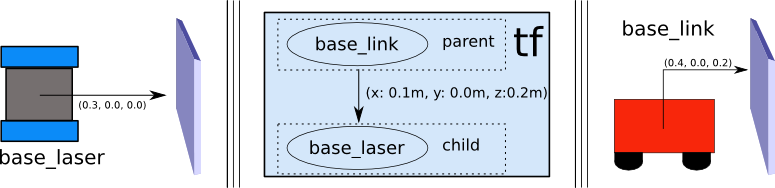
\includegraphics[width=0.5\textwidth,angle=0]{tutorials/tutorial_2/img/tf_robot.png}